\documentclass[12pt]{article}
\usepackage{enumerate}
\usepackage{amsmath}
\usepackage{amssymb}
\usepackage{amsthm}
\usepackage{etoolbox}
\usepackage{graphicx}

\newcommand{\Name}[1]{\noindent \textbf{Name:} #1 \\}
\newcommand{\Workedwith}[1]{\noindent \textbf{Worked with:} #1 \\}
\newcommand{\Problem}[3]{\mbox{} \newline \noindent \textbf{\textbf{Problem #1: #2 [#3 Points] \\ }}}


\begin{document}

\begin{center}
  \bf
  Algorithms \\
  CMPT 307 D200 \\
  Spring 2024 \\
  \rm
  Homework 5\\
  Due:  Sunday, Mar 31 at 10:00 PM \\
\end{center}

\Name{Your name here}
\Workedwith{Everyone you worked with here}

\Problem{4}{Maxiclip}{20}

Many puzzles can be solved by transforming (or ``reducing'') them to network flow problems.  That's what you'll do here!

Maxiclip, a provider of popular online games, has developed a board game that works like this:  We're given an $n \times n$ board.  Some of the squares are gray and the rest are white.  The goal is to place $n$ tokens on white cells such that every row contains exactly one token and every column contains exactly one token.  Tokens may not be placed on the gray cells.
For example, Figure~\ref{fig:boardgame} shows a board with a valid placement of tokens (indicated by the X marks).

\begin{figure}[h]
\begin{center}
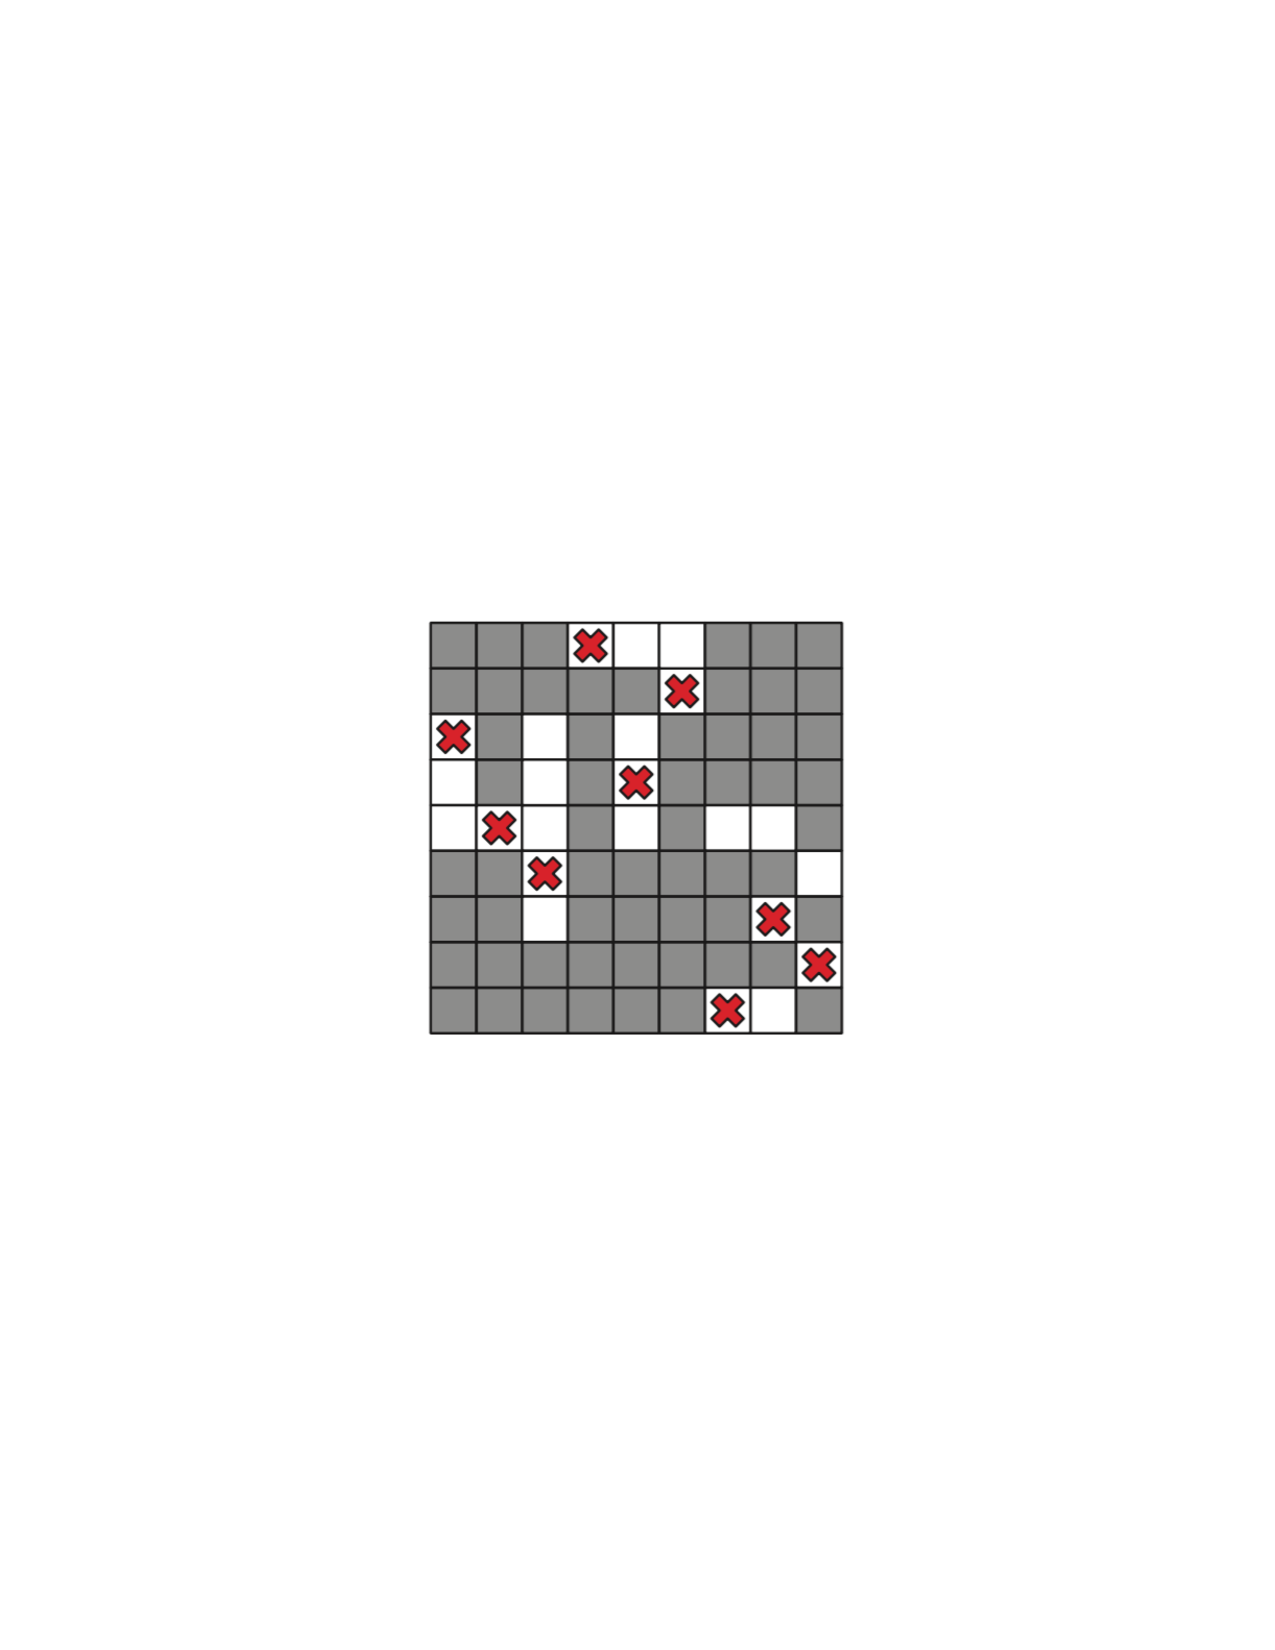
\includegraphics[width=2in]{Board.pdf}
\end{center}
\caption{A square board with a valid placement of tokens.}
\label{fig:boardgame}
\end{figure}

You may assume that the board is represented as follows:  We're given the value of $n$ (the width and heigh to the board) and a list of ordered pairs, each representing the row and column of a white cell in the board.
Using either the Ford-Fulkerson algorithm or the Edmonds-Karp algorithm, describe an efficient algorithm that determines whether or not a given board has a valid solution.  (You don't need to actually give the valid solution if it exists, although you'll see that this is not hard once you can determine whether or not a solution exists.)  Prove that your algorithm is correct and derive its running time as a function of $n$ (and only $n$ -- do not include other terms in the running time).

\textbf{Solution:}
% SOLUTION GOES HERE


\end{document}
